%% LaTeX-Beamer template for KIT design
%% by Erik Burger, Christian Hammer
%% title picture by Klaus Krogmann
%%
%% version 2.1
%%
%% mostly compatible to KIT corporate design v2.0
%% http://intranet.kit.edu/gestaltungsrichtlinien.php
%%
%% Problems, bugs and comments to
%% burger@kit.edu

% remove handout for pauses
\documentclass[18pt]{beamer}

% turn on handout
%\documentclass[handout]{beamer}


%% SLIDE FORMAT

% use 'beamerthemekit' for standard 4:3 ratio
% for widescreen slides (16:9), use 'beamerthemekitwide'

\usepackage{templates/beamerthemekit}
\usepackage{color}

\definecolor{red}{rgb}{1, 0, 0}
\definecolor{blue}{rgb}{0, 0, 1}
\definecolor{green}{rgb}{0, 1, 0}
\definecolor{kitgreen}{RGB}{0, 150, 130}

% \usepackage{templates/beamerthemekitwide}

%% TITLE PICTURE

% if a custom picture is to be used on the title page, copy it into the 'logos'
% directory, in the line below, replace 'mypicture' with the 
% filename (without extension) and uncomment the following line
% (picture proportions: 63 : 20 for standard, 169 : 40 for wide
% *.eps format if you use latex+dvips+ps2pdf, 
% *.jpg/*.png/*.pdf if you use pdflatex)

\titleimage{h2t_title}

%% TITLE LOGO

% for a custom logo on the front page, copy your file into the 'logos'
% directory, insert the filename in the line below and uncomment it

\titlelogo{h2t}

% (*.eps format if you use latex+dvips+ps2pdf,
% *.jpg/*.png/*.pdf if you use pdflatex)

%% TikZ INTEGRATION

% use these packages for PCM symbols and UML classes
% \usepackage{templates/tikzkit}
% \usepackage{templates/tikzuml}

% the presentation starts here

\title[Introducing TensorFlow to H2T]{Introducing TensorFlow to H2T}
\subtitle{}
\author{Jonas Rothfuss, Fabio Ferreira}

\institute{High Performance Humanoid Technologies (H2T)}



% Bibliography
\usepackage[citestyle=authoryear,bibstyle=numeric,hyperref, backend=biber]{biblatex}

\addbibresource{tensorflow.bib}
\bibhang1em


\begin{document}
% change the following line to "ngerman" for German style date and logos
\selectlanguage{english}

%title page
\begin{frame}
\titlepage
\end{frame}

%table of contents
\begin{frame}{Outline}
\tableofcontents

\end{frame}

\section{Overview}
\begin{frame}{Overview}
TensorFlow\footnotemark is a symbolic open-source software library for numerical computation using data flow graphs (\cite{tensorflow})

\footnotetext[1]{TensorFlow, the TensorFlow logo and any related marks are trademarks of Google Inc.}
\begin{itemize}
\item suitable for both research \& production
\pause
\item currently available for Python, C/C++ and Java 
\pause
\item embedded applications: Mobile TensorFlow (Raspberry Pi, Android, iOS)
\end{itemize}
\end{frame}

\begin{frame}{Overview}
\begin{itemize}
\item CPU support
\item GPU support for Nvidia GPUs (requires CUDA and cuDNN) 
\pause
\item for installation see: \textcolor{kitgreen}{ \href{https://www.tensorflow.org/install/install_linux}{[tensorflow manual]}}
\item for workstations@H2T see:
\textcolor{kitgreen}{ \href{https://i61wiki.itec.uka.de/redmine/projects/deeplearning-h2t/wiki/Wiki}{[H2T Deep Learning Wiki]}}
\end{itemize}
\end{frame}

\begin{frame}{Preliminary}
\begin{block}{Best Practices}
\begin{itemize}
\item use Python's \emph{virtualenv} along with pip
\pause
\item if your environment allows it: use \emph{Docker} images (not at H2T)
\pause
\item use \emph{tcmalloc} (memory allocator for high concurrency situations) for a tremendously more efficient resource allocation during training
\end{itemize}
\end{block}
\begin{itemize}
\item for more Best Practices, see: \textcolor{kitgreen}{\href{https://i61wiki.itec.uka.de/redmine/projects/deeplearning-h2t/wiki/Best_Practices}{H2T Deep Learning Wiki}}
\end{itemize}
\end{frame}


\section{Symbolic Programming}
\begin{frame}{TensorFlow's Symbolic Programming}
Two distinctive phases during development:
\begin{block}{symbolic programming paradigm}
\begin{itemize}
\item \textbf{phase 1}: build a computation graph of operations
\pause
\item \textbf{phase 2}: convert the graph into a function (compilation) and execute it in a session
\pause
\end{itemize}
\end{block}
(Bad) consequences:
\begin{itemize}
\item computation happens as the last step in the code
\pause
\item debugging code is usually difficult
\pause
\item native python statements must be provided in TensorFlow language
\pause
\item special statements for typical control flow e.g. \textit{tf.while\_loop}
\end{itemize}
\end{frame}


\begin{frame}{TensorFlow's Symbolic Programming}
Two distinctive phases during development:
\begin{block}{symbolic programming paradigm}
\begin{itemize}
\item \textbf{phase 1}: build a computation graph of operations
\item \textbf{phase 2}: convert the graph into a function (compilation) and execute it in a session
\end{itemize}
\end{block}
(Good) consequences :
\begin{itemize}
\item execution is efficient (memory, in-place computation)
\pause
\item preprocessing and data loading is simply done by adding operations to graph
\pause
\item distribute computation among different resources (multi-gpu, clusters)
\end{itemize}
\end{frame}


\begin{frame}{TensorFlow's Symbolic Programming}
Some TensorFlow terminology first before showing some example code:
\begin{block}{Definition}
\textbf{Tensor}: Is a typed (float32, int32, string) multi-dimensional array. 
\end{block}
For example a mini-batch of 1-channel-images as a 2D-array of floating point numbers with dimensions [batch, width*height]:

\begin{center}
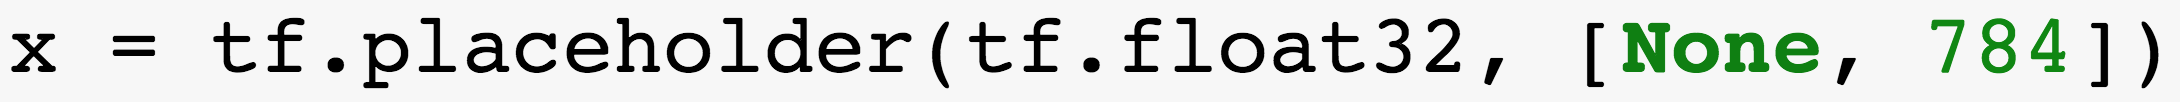
\includegraphics[scale=0.3]{figures/tensor.png}
\end{center}
\end{frame}

\begin{frame}{TensorFlow's Symbolic Programming}
\begin{block}{Definition}
\textbf{Tensor}: Is a typed (float32, int32, string) multi-dimensional array. 
\end{block}
Some widely used types are:
\emph{tf.Variable:}
\begin{itemize}
\item initial values are required
\item for parameters to learn (and save/restore)
\end{itemize}
\emph{tf.Placeholder:}
\begin{itemize}
\item initial values are \emph{not} required
\item for the allocation of storage
\end{itemize}

\end{frame}




\begin{frame}{TensorFlow's Symbolic Programming}
\begin{block}{Definition}
\textbf{Operation}: A node in the computation graph. Takes zero or more Tensors as input, performs computations with them and produces zero or more Tensors.
\end{block}
for example assign a matrix multiplication operation/node to the graph:
\begin{center}
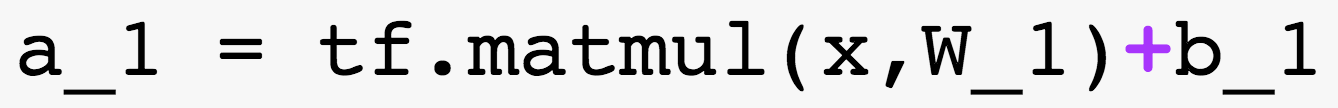
\includegraphics[scale=0.3]{figures/operation.png}
\end{center}
\end{frame}


\begin{frame}{TensorFlow's Symbolic Programming}
\begin{block}{Definition}
\textbf{Session}: For any computation, a graph must be launched in a Session. The Session places the graph onto CPUs or GPUs and provides methods to execute it. Methods executed in a Session return Tensors produced by ops as \textbf{numpy ndarray} objects.
\end{block}
Launch the (default) graph by initializing a session:
\begin{center}
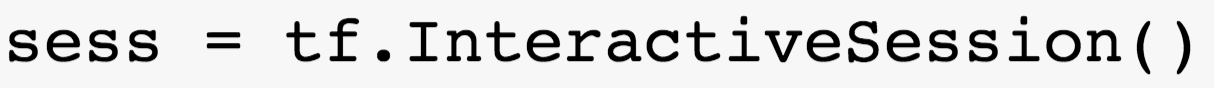
\includegraphics[scale=0.3]{figures/sess1.png}
\end{center}
Calling run() will execute all specified operations in the graph:
\begin{center}
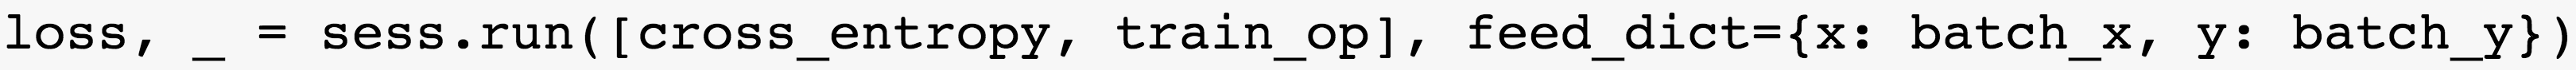
\includegraphics[scale=0.21]{figures/sess2.png}
\end{center}
\end{frame}

\begin{frame}{TensorFlow's Symbolic Programming}
An exemplary graph with input, neurons (weights, biases), softmax and cross entropy function:
\begin{center}
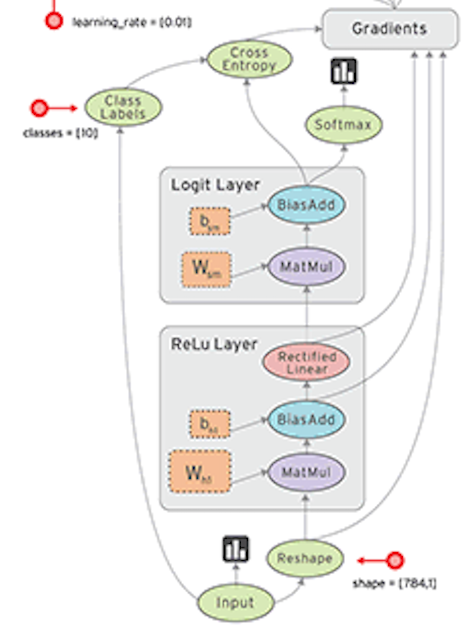
\includegraphics[scale=0.55]{figures/graph.png}
\end{center}
\end{frame}

\section{Example}
\begin{frame}{Workflow of training a NN}
\begin{center}
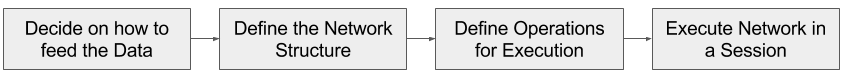
\includegraphics[scale=0.4]{figures/tensorflow_workflow.png}\\Try out the enclosed example code by running the script \emph{start\_tutorial} from the command line. 
\end{center}
\end{frame}


\section{Input pipelines}
\begin{frame}{Data Pre-Processing}
Our main advice for dealing with data is to invest a decent amount of time (25-30\% of total project time) into pre-processing. Here are some questions you should ask (and potential advices in brackets):
\begin{itemize}
\item \textbf{Is the dataset large enough or will I need data augmentation?}
\\($\rightarrow$ plan in more time if it's too small, validate your augmentation by writing test methods for the functions)
\pause
\item \textbf{How likely will I work with more than one dataset?}\\ ($\rightarrow$ think about a uniform dataset pipeline, use tf.flags for differing between datasets) 
\pause
\item \textbf{Which use-cases (e.g. just training a NN, I/O pipeline for a robot demo) will I be confronted with?} \\($\rightarrow$see next two slides)
\end{itemize}
 \end{frame}


\begin{frame}{Three Ways of Importing Data}
Three main ways exist to reading data into TensorFlow:
\begin{itemize}
\item \textbf{Feeding}: Python code provides a sample from data every single iteration
\pause
\item \textbf{Reading}: use an input pipeline for reading the data from files (typically .tfrecords, .csv or binary/encoded data), data fetching is incorporated into the computation graph
\pause
\item \textbf{Preloaded Data}: load a (small) data set entirely into the memory by using constants or variables
\end{itemize}
See the \textcolor{kitgreen}{ \href{https://www.tensorflow.org/versions/r1.2/programmers_guide/reading_data}{[full documentation for Reading Data]}}.
\end{frame}


\begin{frame}{Three Ways of Importing Data}
When to use what?
\begin{itemize}
\item use \textbf{Feeding} 
\begin{itemize}
\item to get familiar with TensorFlow
\item for live-demos
\item for tunneling data through third-party services/pipelines (e.g. ICE)
\end{itemize}   
\pause
\item use \textbf{Reading}  if
\begin{itemize}
\item your data set is too large to be stored in the memory directly
\item you need to efficiently train a NN
\item you want to benefit from native pipeline functions (e.g. automatic batch-creation/-handling, Threading \& Queuing)
\end{itemize}
\pause
\item use \textbf{Preloaded Data} if 
\begin{itemize}
\item your data set is small enough to be stored in the memory directly
\item you want efficiency in training an NN and
\item benefit from the the native pipeline (see \emph{Reading})
\end{itemize}
\end{itemize}
\end{frame}


\begin{frame}{Importing Data with the Dataset API}
TF has recently (r1.2.) introduced a new \textcolor{kitgreen}{ \href{https://www.tensorflow.org/programmers_guide/datasets}{Dataset API}} for dealing with large amounts of data, different file formats and transformations (e.g. batches) which also incorporates Threading \& Queuing. If you want to use \emph{Dataset}, principle steps are:
\begin{itemize}
\item \textbf{Decide on the abstraction level}: \emph{tf.data.Dataset} is a sequence of elements and every element contains one or more Tensors (e.g. in an image pipeline every element is a single image)
\pause
\item \textbf{Define the source of your data set}: to start an input pipeline, you must specify a source, e.g. by loading the Tensors from memory or TFRecords
\pause
\item \textbf{Apply transformation}: once a source is defined, you can transform the Dataset into a new Dataset that suffices your requirements (e.g. creating a batch or using \emph{Dataset.map()} to apply a function to each element)
\end{itemize}
Existing (old) Input Pipeline methods will be available until TF 2.0 (at least).
\end{frame}


\begin{frame}{TensorFlow's TFRecords}
TFRecords is a supported format for any type of data. Creating the records can sometimes be a hassle but once they exist you'll benefit from helpful native pipeline functions. \\[12pt]For generating TFrecords one ideally writes a (1st) routine that:
\begin{itemize}
\item reads-in the data (e.g. 3 channel image in numpy array)
\item place the data into a protocol buffer \emph{tf.Example} object
\item serializes the protocol buffer into a string
\item writes the string into a TFRecords file using the \emph{tf.TFRecordWriter}
\end{itemize}
\end{frame}

\begin{frame}{TensorFlow's TFRecords}
On the other side, to use the generated TFRecords, one writes a (2nd) routine that:
\begin{itemize}
\item reads-in the records with \emph{tf.TFRecordReader} 
\item decodes the data with \emph{tf.parse\_single\_example} to receive the deserialized data as a tensor for a single sample
\item uses the tensor as a template to create a batch for training \emph{tf.train.batch}
\item next, choose the size of the batch (how many of template tensors need to be in a batch) to receive a new tensor (representing the batch) 
\item provides the new tensor to the model at initialization (before \emph{sess.run()}
\end{itemize}


Examples can be found \textcolor{kitgreen}{ \href{https://github.com/jonasrothfuss/DeepEpisodicMemory/blob/master/data_prep/convertToRecords.py\#L60}{here (Deep Episodic Memory)}} and \textcolor{kitgreen}{ \href{https://www.tensorflow.org/api_guides/python/reading_data\#file_formats}{here (TensorFlow doc)}}.

\end{frame}



\section{Useful remarks}
\begin{frame}{Useful remarks: Save \& Restore a Graph}
Saving \& restoring a graph is
\begin{itemize}
\item typically useful when a training should be saved, e.g. after 1000 training iterations / 1 hour
\item or if you want your results to be reproducible
\end{itemize}

\textbf{For saving \& restoring examples}: see \textcolor{kitgreen}{ \href{https://github.com/jonasrothfuss/DeepEpisodicMemory/blob/master/train_model.py\#L320}{here (Deep Episodic Memory)}} and \textcolor{kitgreen}{ \href{https://www.tensorflow.org/programmers_guide/saved_model}{here (TensorFlow doc)}}.

\textbf{Fine-tuning a pre-trained model:} this has touching points with the saver. If you need to exclude some variables from the graph for training,  see \textcolor{kitgreen}{ \href{https://github.com/jonasrothfuss/DeepEpisodicMemory/blob/master/train_model.py\#L249}{this code}}.

\textbf{Recommended}: create a protocol of parameters (solver, output directory, dataset etc.) you specified for your trainings, e.g. as done \textcolor{kitgreen}{ \href{https://github.com/jonasrothfuss/DeepEpisodicMemory/blob/master/utils/io_handler.py\#L201}{here}} or directly use config files.
\end{frame}


\begin{frame}{Useful remarks: Visualization}
Visualization can help track down problems in your architecture/code but can also help doing sanity checks and help monitoring the training progress. Visualization is done with TensorBoard. \\[8pt]
\begin{itemize}
\item \textcolor{kitgreen}{ \href{https://www.tensorflow.org/get_started/graph_viz}{Graph Visualization}} (can help finding structural errors when code is already to complex)
\item \textcolor{kitgreen}{ \href{https://www.tensorflow.org/get_started/summaries_and_tensorboard}{Visualizing Learning}} (monitor your training progress)

\begin{center}
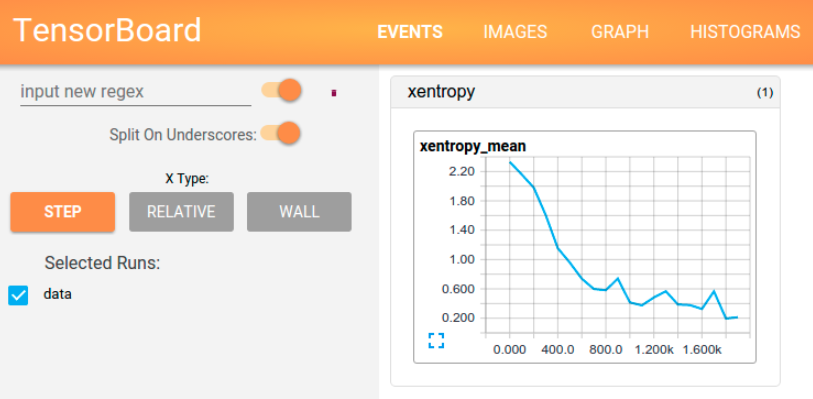
\includegraphics[scale=0.2]{figures/tensorboard.png}
\end{center}
\end{itemize}
You can access TensorBoard via ssh from different computers, see \textcolor{kitgreen}{ \href{https://github.com/jonasrothfuss/DeepEpisodicMemory/blob/master/commands.md}{here}}
\end{frame}


\begin{frame}{Useful remarks: Debugging}
Due to symbolic programming, debugging TensorFlow programs is generally hard. To make things easier, the authors have introduced two helpful tools:\\[8pt]
\begin{itemize}
\item \textcolor{kitgreen}{ \href{https://www.tensorflow.org/programmers_guide/debugger}{TensorFlow debugger (tfdbg)}}: debug-wrapper around \emph{sess.run()} that allows a program to start with \emph{--debug} flag $\rightarrow$ interactive debug mode in console
\item newly introduced: \textcolor{kitgreen}{ \href{https://github.com/tensorflow/tensorflow/blob/master/tensorflow/contrib/eager/README.md}{TensorFlow Eager Execution}}, an interface for imperative programming style. Activate eager execution and execute TF operations immediately without executing a graph with \emph{sess.run()}
\end{itemize}
\end{frame}

\section{Conclusion}
\begin{frame}{Concluding}
Things we considered most challenging during Deep Episodic Memory
\begin{block}{Challenges}
\begin{itemize}
\item setting-up the training pipeline with tfrecords
\pause
\item keeping track of changes and decisions that affected the design of the model
\pause
\item finding bugs (or assess the effect of code changes) in symbolic programming
\end{itemize}
\end{block}
\end{frame}




\appendix
\beginbackup

\begin{frame}[t,allowframebreaks]{References}
\printbibliography
\end{frame}

\backupend

\end{document}
